\documentclass[]{rsos}%%%%where rsos is the template name

%%%% *** Do not adjust lengths that control margins, column widths, etc. ***


%%%%%%%%%%% Defining Enunciations  %%%%%%%%%%%
\newtheorem{theorem}{\bf Theorem}[section]
\newtheorem{condition}{\bf Condition}[section]
\newtheorem{corollary}{\bf Corollary}[section]
%%%%%%%%%%%%%%%%%%%%%%%%%%%%%%%%%%%%%%%%%%%%%%%



\begin{document}

%%%% Article title to be placed here
\title{Zebrafish survival depends on escaping predators from a distance}

\author{%%%% Author details
Arjun Nair, Christy Nguyen, and Matthew J. McHenry}

%%%%%%%%% Insert author address here
\address{Department of Ecology and Evolutionary Biology\\
University of California, Irvine\\
321 Steinhaus Hall\\
Irvine, CA 92697}

%%%% Subject entries to be placed here %%%%
\subject{Animal behavior, biomechanics}

%%%% Keyword entries to be placed here %%%%
\keywords{pursuit-evasion model, locomotion, predation, sensing, strategy}

%%%% Insert corresponding author and its email address}
\corres{Matthew J. McHenry\\
\email{mmchenry@uci.edu}}



%%%%%%%%%%%%%%% End of first page %%%%%%%%%%%%%%%%%%%%%

\maketitle

%%%%%%%%%% Insert the texts which can accomdate on firstpage in the tag "fmtext" %%%%%

%\begin{fmtext}


\linespread{1.6}\selectfont %Doublespacing


\section*{Abstract}
Predation is a fundamental interaction between animals, yet it is largely unclear how sensing and locomotion allow prey to survive encounters with predators.
Using experiments and pursuit-evasion modeling, we examined the effects of kinematic events on prey survival in interactions between zebrafish (\textit{Danio rerio}) larvae and predators  (adults and juveniles) of the same species.
High-speed 3D kinematic measurements tracked the body position of prey and predator to determine the probabilities of behavioral events by both fish.
These measurements provided the basis for a pursuit-evasion model that simulated the trajectories of predator and prey. 
The model was verified by the measured number of strikes that prey survived before capture.
We conducted a sensitivity analysis of the model to determine which kinematic events influence prey survival.
Our results suggest that zebrafish prey enhance survival only by expanding their reaction distance and that similar benefits cannot be achieved by increasing speed or altering the direction of an escape.
Therefore, larval zebrafish escape with sufficient speed, but would benefit from responding from a greater distance.
These findings suggest that the performance of predator detection is the decisive factor in the survival of fish prey.
The suite of physiological characteristics that enable predator sensing should therefore distinguish successful prey and play a major role in the evolution of prey strategy.

\section{Introduction}

Predator-prey interactions offer a behavioral context for understanding the biomechanics and neurophysiology of animals.
It is commonly argued that the survival of evasive prey and the success of predators depend on fast or highly-maneuverable locomotion \cite{Alexander:BbR35qCj, Wilson:2013fda, Walker:2005vn, Domenici:2011tv, Howland:1974ud}, the rate and force of predatory strikes \cite{deVries:2012tc, Holzman:2009uu}, and the ability of prey to sense an approaching predator at great distance \cite{Dill:1972wh, Gabbiani:1999wz}.
However, it is not clear how these factors compare in strategic importance and it is consequently unknown what traits distinguish successful prey. 
The aim of the present study was to determine the kinematic parameters that are most important in determining the survival of a fish when it becomes the prey of a larger fish.

Experimental approaches for understanding the dynamics of predators and prey are challenged by the interdependency of both animals' actions.
Any motion by the prey may (or may not) be in response to the predator, which may (or may not) be a response to prior motion by the prey. 
This behavioral coupling has the potential to make the actions of both animals appear as a stochastic chain of events.
Multivariate statistics are generally insensitive to such dynamics, yet may succeed in resolving dominant features of successful prey \cite{Walker:2005vn} or predators \cite{Wainwright:2001ufa}.
Such analysis is enhanced by considering behavioral responses to an artificial predator or prey that is experimentally controlled and therefore not coupled \cite{Gabbiani:1999wz,Stewart:2014cma,Heuch:2007kk}.
An alternative approach attempts to formulate a behavioral algorithm of one animal by considering their responses to the measured kinematics of the other.
For example, such an approach found that predatory bats track evasive moths by maintaining their heading, rather than attempting to anticipate the prey's direction \cite{Ghose:2006dk}. 
The present study introduces a variant on this technique by pairing kinematic analysis of predator and prey with pursuit-evasion modeling to examine the effects of kinematic parameters on predictions of prey survival.

Pursuit-evasion models consider the interactions between predator and prey by simulating how both animals move through space.
This application of pursuit-evasion models has addressed the optimal direction of escaping fish prey \cite{Weihs:1984tb} by assuming simplified kinematics.
From this perspective, predator-prey strategy may be categorized by the speed of the predator relative to the prey \cite{Soto:2015cj}. 
The fast-predator domain corresponds to situations where the predator approaches at 10-times the escape speed of the prey.
In this domain, the escape direction may matter little because of the meager distance that the prey may attain before being overtaken by the predator.
In the slow-predator domain, where prey are faster than the predator, the rapid escape of prey permits a broad range of escape directions that are equally effective.
It is only in the intermediate domain, when the predator is slightly faster, that the prey benefits by conforming to an optimal strategy.
Prey operating in any domain should benefit from initiating an escape from a greater distance.
These pursuit-evasion models offer a heuristic framework, but it is unclear how predictive they may be for biological systems. 
For example, these models generally assume that both predator and prey operate with perfect information and move with a constant velocity and heading in purely deterministic calculations that do not consider variable behavior.
In the interest of creating a pursuit-evasion model that is representative of realistic predator-prey interactions, we presently developed a pursuit-evasion model that incorporates measured variation in kinematic events in simulations that predict the motion of predator and prey. 

We performed our study with a focus on zebrafish (\textit{Danio rerio}). 
The larval stage of this species serves as a model for studying the neurophysiological \cite{Bianco:2015gm,Bagnall:2014iu,Huang:2013vj} and biomechanical \cite{Muller:2004hp,Li:2016cy} basis of behavior.
Predator-prey interactions may be experimentally replicated in the lab, where adults and juveniles strike at larvae with suction feeding and the larvae respond with a fast-start escape response \cite{Stewart:2013bha}.
These are the two principle behaviors that characterize of a broad diversity of piscivorous interactions \cite{Weihs:1984tb,Walker:2005vn,Higham:2007go,Higham:2005iu}. 
When approaching an evasive prey, zebrafish predators will approach much more slowly than their maximum speed.
This is a common phenomenon among suction-feeding fishes \cite{Higham:2005iu,Higham:2007go}, perhaps because it allows greater control over the direction and timing of the strike.
Suction feeding is limited to a brief duration over a small region in front of the mouth \cite{Holzman:2008jc,Holzman:2009uu}. 
In contrast, the high speed of the fast-start escape permits zebrafish larvae to operate in the slow-predator domain, where they may successfully escape in a variety of directions \cite{Soto:2015cj}.
We tested this prediction of pursuit-evasion models and additionally examined how prey survival depends on the reaction distance and speed of the escape.  
We performed experiments both with juvenile and adult predators to examine how the strategy of prey may vary with the relative size of the predator \cite{Fuiman:1994td}.


\section{Material and methods}

\subsection{Animal husbandry}
All experiments were conducted on zebrafish (\textit{Danio rerio}, Hamilton 1922) with larvae (5 -- 7 days post fertilization, dpf) that were preyed upon by older fish of the same species. 
To examine how these interactions vary with the size of the predator, we performed one set of experiments using adults ($\geq 9$ months old, $3.4 \pm \SI{0.5}{\cm}$, \textit{N} = 19) and another using juvenile predators ($3-4$ months old, $2.0  \pm  \SI{0.4}{\cm}$, \textit{N} = 19).
All fish were bred from wild-type (AB line) colonies housed in a flow-through tank system (Aquatic Habitats, Apopka, FL, USA) that was maintained at $\SI{28.5}{\celsius}$ on a 14:10 h light:dark cycle. 
To produce larvae, the fertilized eggs from randomized mating were cultured according to standard techniques \cite{Westerfield:UXiBrEuA}.
Predators were motivated to feed by fasting for a period of 7 -- 14 days prior to an experiment.


\subsection{Kinematics}
We arranged the lights and cameras for high-speed recordings of both fish with high-contrast images. 
A hemispherical aquarium ($\oslash = \SI{8.5}{\cm}$) was composed of white acrylic, which served as a translucent diffuser of the IR illumination (940 nm) provided by three lamps (CM-IR200-940, CMVision, Houston, TX, USA), positioned below (Fig. \ref{fig_setup}a). 
These lamps provided high-intensity illumination that was invisible to the fish \cite{Robinson:1993tu}, while visible illumination at low intensity was provided by overhead fluorescent lights.
Each camera (FASTCAM Mini UX50, Precision Photron Inc., San Diego, CA, USA) was fitted with a \SI{55}{\mm} lens (f/2.8 Micro Nikkon AIS, Nikon Inc., Melville, NY, USA) and positioned at a distance that permitted a view of the entire aquarium. 
The cameras were angled above the aquarium to allow both fish to be viewed by at least two cameras when the fish were positioned close together, despite the aquarium walls blocking the view of the two fish.
The cameras were synchronized to record at a 1,000 fps (at 1024 x 1024 pixels) with a common TTL trigger and controlled with the manufacturer's software (PhotronFASTCAM Viewer).

Predation experiments were performed by recording the swimming of one predator and one prey fish in the aquarium (Fig. 1A). 
This began by placing the fish on opposite sides of a partition.
Following a \SI{15}{\min} acclimation period, we lifted the partition and observed the fish until the predator successfully ingested the prey.
Using a end-trigger to the high-speed cameras, we saved recordings from $\sim \SI{0.5}{\s}$ before the first predatory strike and until $\sim \SI{0.5}{\s}$  after the prey was captured.

Our video recordings were used to perform measurements of 3D kinematics. 
We calibrated the cameras by recording a static body that we constructed with 48 landmarks of known relative position, which was placed in the center of the aquarium.
A direct-linear transform (DLT) was calculated using `Digitizing Tools' software in MATLAB (2015a, MathWorks, Natick, MA, USA) \cite{Hedrick:2008wz} from manually-selected coordinates of these landmarks from the perspective of the three cameras.
Using a custom script in MATLAB, we found the body positions of predator and prey fish by selecting landmarks from two camera views and using the DLT to determine the coordinates in 3D space.
We used the position of the predator's two eyes to calculate a mean position that approximated the buccal cavity (Fig. \ref{fig_setup}a).
The posterior margin of the swim bladder was found on the prey's body, which approximates the center of mass \cite{Stewart:2010ig}.
The initial heading of the prey was approximated by matching an ellipsoid (using 'regionprops' method in MATLAB) to the body of the prey and measuring the angle of the major axis of the ellipsoid.
All subsequent heading measurements of the prey was defined as the average angular displacement of prey during an escape and was relative to the previous heading of the prey.
We acquired the landmark positions at four key events in each interaction between predator and prey: (1) when the predator initiated an approach toward the prey, (2) at the mid-duration of suction feeding by the predator and (3) at the initiation and (4) completion of the prey's escape response.


\subsection{Descriptive statistics}

Descriptive statistics were used to characterize the probability of actions by the predator and prey during predation experiments.
For all interactions recorded among our experiments, we found predator-specific parameters that consisted of the strike distance ($s$), the distance from the prey at which a strike was initiated, and the strike duration ($\tau$), which was defined as the period between the opening and closing of the mouth during suction feeding. 
For the prey, we found the reaction distance ($l$), the distance from the predator at which the escape response was initiated.
The prey's kinematics were additionally characterized by the escape angle ($\theta$), the angular change in heading from the resting orientation to the escape path.
The escape duration ($\eta$) included the period for all stages of the C-start and subsequent undulatory swimming, until the larva ceased moving.
The frequency distribution for each parameter was found to be well-approximated by the following lognormal probability density function:
%
\begin{equation}%%% Equation lognormal distribution
f(x) = \frac{1}{x\sigma \sqrt{2 \pi}} \text{exp} \left[ -{\frac{(ln(x)-\mu)^2}{2\sigma ^2}} \right],
\label{eqn_lognorm}
\end{equation}
%
where $x$ is a particular behavioral parameter ($s, \tau, l, \theta ,$ or $\eta$), $\mu$ is the log mean, and $\sigma$ is the log standard deviation. 
We determined best-fit values for $\mu$ and $\sigma$ for each behavioral parameter by maximum-likelihood (the `fitdist' function in MATLAB).

The probability that the strike of a zebrafish predator is successful depends critically on the distance between the mouth of the predator and the prey \cite{Stewart:2013bha}.
Strikes were therefore measured as a function of distance. 
These measurements revealed that the probability of a successful capture $(C)$ was well-characterized by the following sigmoidal function:
%
\begin{equation}%%%Equation for sigmoid function
C(d) = \left[ 1+e^{-r(d-d_0)} \right]^{-1},
\label{eqn_sig} 
\end{equation}
%
where $d$ is the distance between predator and prey, $d_0$ is the decay distance, and $r$ is the decay rate. 
The best-fit values for $d_0$ and $r$ were determined by least-squares (`sqcurvefit' function in MATLAB).

All parameters for the prey and predators were compared between experiments with adult predators and juvenile predators.
We found that these parameters failed to conform to normal distributions.
We therefore performed comparisons with non-parametric statistics, using a two-sample Kolmogorov-Smirnov test (i.e. KS-test) \cite{MasseyJr:1951jo}. 


\subsection{Pursuit-evasion model}
A pursuit-evasion model was developed to simulate the conditions of our experiments. 
This model predicted the 2D motion of a predator (i.e. pursuer) and prey (i.e. evader) \cite{Isaacs:1965uz} according to algorithms that were specific to the behavioral state of each of these agents (Fig. \ref{fig_setup}b). 
The predator's states were Tracking and Striking and the prey's were Resting and Escaping. 
The duration of states, probability of transitioning between states, and probability of prey capture were determined by random-number generation that conformed to the probability distributions and range of values that we measured.
Therefore, the model treated the predator and prey's actions as probabilistic, but each outcome of an interaction also depended on the determinism of the kinematics of the two agents.
Simulations were scripted in MATLAB to calculate the motion of both agents and their behavioral states, which consequently determined the number of unsuccessful strikes before prey capture.

Each simulation began with the predator in the Tracking state, where it moved at an approach speed with a direction that was always headed toward the prey, with perfect information about the prey's position (Fig. \ref{fig_setup}b). 
If the prey was motionless, then the solver would skip in time to the strike or escape initiation, whichever was found to occur first.
Otherwise, the solver would resolve both predator and prey motion with a fixed time step of \SI{5}{\ms}. 
In this regime, the predator adjusted its heading to track the prey with a temporal time delay, $\lambda$.  
The predator's transition into the Striking state occurred when the prey was within a particular distance that was determined by the strike distance. 
This value was determined \textit{a-priori} by the generation of a random value (using the `random' function in MATLAB) according to the lognormal probability density function (Eqn. \ref{eqn_lognorm}) for measured values of strike distance.
The capture probability, $C$, for a particular strike depended on the distance between the agents in the middle of a strike, according to our measured parameter values for this relationship (Eqn. \ref{eqn_sig}).
This relationship was used to determine whether a strike successfully captured a prey.
The simulation was terminated if a strike was successful, otherwise the predator reverted to the Tracking state after completion of the strike duration (Fig. \ref{fig_setup}b).
The value of strike duration was determined by the generation of a random value from the lognormal probability density function from measured values.
Single values for the predator speed and delay were used for all simulations (Table \ref{table}) and were determined by trial-and-error to replicate the distribution of the measured number of unsuccessful strikes before prey capture. 
These values were found to approximate measurements reported in prior studies \cite{McHenry:2005tc, Stewart:2013bha}. 

The pursuit-evasion model simultaneously determined the actions of prey (Fig. \ref{fig_setup}b).
Prey behavior was modeled with Resting and Escaping states because larval zebrafish generally remain still between periods of rapid swimming initiated by an escape response \cite{Stewart:2013bha, Stewart:2014cma}. 
The prey began each simulation in the Resting state, where it was motionless at a random distance equal to, or less than, the aquarium diameter ($\oslash = \SI{8.5}{\cm}$) away from the predator.
The prey transitioned into the Escaping state when the predator moved within the reaction distance after a latency \cite{Nair:2015gk}.
During an escape, the prey was assumed to follow a straight path in the direction of the escape angle.
Using a frame-by-frame kinematic analysis of escape swimming for 12 larvae, we found that prey varied speed as a saw-toothed function of time that approximately attained its maximum value at 20\% of the duration. 
We consequently modeled variation in swimming speed for prey to attain the maximum speed at 0.2$\eta$, where $\eta$ is the escape duration. 
The reaction distance, escape angle, and escape duration were determined by random numbers with probability density functions matching experimental measurements.
The escape angle was defined with respect to the prey's frame of reference, with $\theta =  \SI{0}{\degree}$ corresponding to forward motion.
The  escape direction was defined as the probability that the escape angle was directed away from the predator, with a value (Table \ref{table}) that was previously measured \cite{Stewart:2014cma}.

This model simplified many aspects of the complexity of predator-prey interactions.
It assumed that the kinematics of the two fish may be approximated with two-dimensional motion that is not bounded by an aquarium. 
Simulations were halted if prey successfully escaped on 20 occasions, which reflected the observed maximum and guarded against an errant simulation of infinite duration.
The model's probabilistic approach considered the probabilistic effects of biomechanics and neurophysiology without explicitly articulating those elements.
For example, capture success was treated as a distance-specific probability (Eqn. \ref{eqn_sig}) that modeled neither the effects of a predator's suction-feeding hydrodynamics, nor the propulsive forces generated by an escaping prey.
The number of successful escapes before capture for all experiments were compared to the same metric for 1,000 simulations.  
This comparison was executed by a two-sample Kolmogorov-Smirnov test, which was chosen over a Kruskal-Wallis test because of its emphasis on the shape of the distribution.  

A sensitivity analysis evaluated the parameters that characterized prey behavior to determine which had the greatest effect on prey survival. 
This was achieved by running batches of a 1,000 simulations where one parameters was varied between -90\% and 100\% of their original mean values at increments of 10\%.
Batches  were ran for each prey associated parameter.
For parameters described by a probability distribution, the log-mean parameter, $\mu$, was adjusted to create the desired percent-change in the mean of the distribution, while $\sigma$ was held constant.
The range of possible random values for each distribution was also adjusted to retain the the same cumulative probability range in the probability distribution.
The effect of these manipulations were assessed by comparing the measured escape probability against the model's prediction using a Kruskal-Wallis test. 



\section{Results} %==================================================================

\subsection{Kinematics} %==========
The behavior of both predator and prey were similar whether the predators were juvenile or adult zebrafish.
Prey responded with similar behavior, having indistinguishable differences in escape angle (KS-test: $P = 0.86, N = 164$) and with modest, though significant, differences in reaction distance (KS-test: $P < 0.001, N = 164$) and escape duration (KS-test: $P = 0.04, N = 153$) (Fig. \ref{fig_PDF}\textit{b--c}). 
For example, prey reacted at a mean distance to juvenile predators ($\overline{l} = \SI{8.4}{\mm}, N = 91$), that was about two-thirds the reaction distance to adults ($\overline{l} = \SI{12.6}{\mm}, N = 73$).
Escape swimming lasted for about one-third of a second, with the response to juveniles ($\overline{\eta} = \SI{0.35}{\s}$, $N$ = 91) being only  $\SI{50}{\ms}$ longer than to adults ($\overline{\eta} = \SI{0.30}{\s}$, $N$ = 62).
Prey escaped earlier to adult predators (KS-test: $P = 0.02, N = 89$) by $\SI{41}{\ms}$, on average, relative to the mid-duration of suction feeding.
Juvenile and adult predators were not significantly different in either their strike distance (KS-test: $P = 0.08, \overline{s} = \SI{7.6}{\mm}, N = 154$), or strike duration (KS-test: $P = 0.87, \overline{\tau} = \SI{44}{\ms}, N = 107$) (Fig. \ref{fig_PDF}\textit{d--e}).
Therefore, much of the behavior of predator and prey were similar, despite the fact that the adults were nearly twice the body length of the juveniles.

Despite having similar behavior, adult and juvenile predators differed in capture performance.
Juveniles did not succeed in capturing prey beyond a distance of $\SI{3.2}{\mm}$ ($N = 91$), whereas adults captured prey at a maximum distance that was about 3-times greater ($\SI{10.4}{\mm}, N = 77$).
In the relationship between capture probability and distance (Eqn. \ref{eqn_sig}), the decay distance was used to indicate the spatial range of high capture probability. 
By this metric, the strike of adult predators also exhibited a range that was slightly greater than 3-times the distance of juveniles (Table \ref{table}, Fig. \ref{fig_PDF}\textit{f}).
We tested whether this result was due to juveniles approaching the prey with inferior accuracy by measuring the bearing angle of predators.
This angle corresponds to the radial position of the prey relative to the predator's heading, such that a predator is perfectly accurate for a prey position of $\SI{0}{\degree}$, and therefore indicated the spatial accuracy of a strike.
The bearing angle when they prey initiated an escape was not significantly different (KS-test: $P = 0.15$) between juveniles ($N = 91$) or adults ($N = 77$).
However, bearing angles changed such that there was a significant difference (KS-test: $P = 0.15$) between adults and juveniles when measured at the moment of mid-gape.
Adult predators succeeded in achieving a median bearing of $\SI{13.1}{\degree}$ (Mean = \SI{35.3}{\degree}), whereas the same metric was $\SI{30.0}{\degree}$ (Mean = \SI{39.2}{\degree}) in juveniles.
This suggests that adults were more accurate in their strikes and more effectively adjusted their heading in the time between escape and strike.


\subsection{Pursuit-evasion model} %==========
The trajectories of predator and prey fish followed paths that were qualitatively similar to that predicted by our pursuit-evasion model.
For most of the duration of our experiments, predators were observed to be swimming toward the prey (Fig. \ref{fig_traj}a). 
In contrast, the prey were generally motionless, except  when executing escape swimming.
The predators and prey followed a more circuitous path in the predation experiments than the motion prescribed by our model (Fig. \ref{fig_traj}b).
Nevertheless, the temporal sequence of events in the model offered a reasonable approximation of the kinematics of live predator-prey interactions.

The model accurately predicted the broad quantitative patterns of our experimental results.
This was assessed by the probability of the prey surviving over a particular number of strikes. 
In our experiments, prey exhibited the greatest probability of being captured on the first strike with monotonically decreasing probabilities over subsequent strikes (Fig. \ref{fig_traj}c).
Adults were more successful on the first, second and third strikes than juveniles, which consequently exhibited a more even probability distribution.
The model was successful in replicating these trends, which were found to be statistically indistinguishable for both adult (KS-test: $P = 0.93, N = 73$) and juvenile (KS-test: $P = 0.86, N = 91$) predators. 
Furthermore, all trends from the sensitivity analyses of the pursuit-evasion model were similar between the adult (Fig. \ref{fig_sense}) and juvenile (Fig. S1) predators. 

A sensitivity analysis of prey parameters revealed that escape speed and reaction distance were the only parameters with a substantial effect on prey survival. 
This result was determined by adjusting the probability distribution of each parameter to generate a percent change in the mean value of that parameter among 1,000 simulations.
Generating these changes in escape duration, escape direction, and escape angle led to statistically insignificant or small changes in escape probability (Fig. \ref{fig_sense}a). 
An increase in escape speed similarly had a negligible effect on survival, but survival probability did decline when speed was reduced by 50\% or more.
However, survival was most sensitive to reaction distance.
Increases to the mean reaction distance caused escape probability to increase up to 16\% and decreases in the mean reaction distance by 30\% or more had a dramatic adverse effect on survival (Fig. \ref{fig_sense}a). 

We examined how the effect of reaction distance varies with escape speed by conducting a two-dimensional sensitivity analysis (Fig. \ref{fig_sense}\textit{b}).
It was not until speed was reduced by more than 50\% that the relationship between response distance and survivor was altered.
For example, reducing speed by 70\% yielded a distinct curve, the shape of which was similar to the sigmoid generated at higher speeds (Fig. \ref{fig_sense}\textit{c}). 
Alterations in response distance did affect the relationship between escape speed and survival , though the shape of this curve was largely unaltered (Fig. \ref{fig_sense}\textit{d}).
This suggests little evidence for an interactive effect on survival between escape speed and response distance.



\section{Discussion}%================================

The present study succeeded in testing how a prey's kinematics affect their ability to survive an encounter with a predator.
This was achieved by developing a pursuit-evasion model that successfully replicated the broad patterns of survival (Fig. \ref{fig_traj}\textit{c}) by incorporating the measured probabilities of behavioral events in zebrafish (Fig. \ref{fig_PDF}).
A sensitivity analysis of the model revealed that prey may improve survival only by expanding the distance at which an escape is initiated (Fig. \ref{fig_sense}). 
The observed escape speed is sufficiently rapid and the escape may be successfully executed in a variety of directions.
These results were largely similar whether the predator was a juvenile or adult zebrafish.


\subsection{Prey survival depends on reaction distance} 

Our finding on the importance of reaction distance is consistent with prior theoretical and experimental studies.
The reaction distance commonly serves as a metric of the sensitivity of prey to an approaching predator in behavioral ecology studies \cite{Cooper:2015vf}.
The strategic advantage to responding at a greater distance is supported by the predictions of pursuit-evasion models, particularly in models were both animals are assumed to maintain a fixed heading \cite{Isaacs:1965uz,Weihs:1984tb,Soto:2015cj}. 
Quite simply, a prey's ability to maintain some distance is enhanced when they start from further away.

However, there are a variety of conditions where one might expect a response from a great distance to have adverse consequences.
Ydenberg and Dill \cite{Ydenberg:1986tm} illustrated a myriad number of ways in which escaping in response to a predator may incur costs that exceed the benefits of predator evasion.
For example, escape responses may be energetically costly, prohibit foraging, or succeed in revealing a cryptic prey \cite{Cooper:2015vf,Broom:2005gq}.
The potential for costs are largely removed in our experiments, where prey are provided little alternative to predator evasion.
However, the costs to escape behavior could have been shaped the evolution of zebrafish behavior.
Responding from a great distance may even be inferior on purely strategic grounds. 
For example, escaping early along a straight path, as we observed in zebrafish larvae (Fig. \ref{fig_traj}\textit{a}), may afford more time for a predator adjust its heading and accelerate to intercept a prey. 
We did not find evidence for this in zebrafish (Fig. \ref{fig_PDF}\textit{f}), but it remains a possibility in other species.

The primacy of escape distance underscores the strategic importance of predator sensing. 
Our model is not explicit about any particular sensory modality, but our measurements of reaction distance (Fig. \ref{fig_PDF}\textit{c}, Table \ref{table}) are within the range possible for vision \cite{Dunn:2016jt}, olfaction \cite{Waldman:1982ic}, or flow sensing by the lateral line system.
Olfactory cues probably did not play a major role in our experiments. 
Zebrafish are sensitive to the smell of the alarm pheromone Schreckstoff, which is released by conspecifics when the skin is damaged. 
However, this sensitivity is not acquired until a later stage in zebrafish growth (>48 dpf) \cite{Waldman:1982ic} and the water in our experimental aquarium was changed between trials.
Our experimental design does allow for the possibility that the scent of adult zebrafish could enhance the sensitivity of other sensory modalities.

Previous work established that escape responses are elicited in larval zebrafish by a looming visual stimulus \cite{Bianco:2011ca} and by the bow wave of flow ahead of an approaching predator \cite{Stewart:2014cma}.
Vision offers superior range, but its demands for neuronal processing necessitate a latency of at least $\SI{200}{\ms}$ \cite{Burgess:2007vp}, in contrast to the rapid responses to flow that may occur in less than $\SI{10}{\ms}$  \cite{Liu:1999fs}.
The flow sensing that is facilitated by the lateral line system is necessary for zebrafish larvae to survive encounters with adult predators \cite{Stewart:2013bha}, but its limited range fails to stimulate an escape response beyond a distance of \SI{1.3}{\cm} \cite{Stewart:2014cma}.
This suggests that the responses at greater distances (Fig. \ref{fig_PDF}\textit{c}, Table \ref{table}) may be attributed to the visual appearance of the predator as a looming stimulus. 
It is at these distances where prey gain the greatest strategic advantage ((Fig. \ref{fig_sense}\textit{a}).
Therefore, our findings suggest that prey have the best change at surviving an encounter with a predator when they are responsive to a threatening visual stimulus.
It follows that the performance of the visual system of prey is the most decisive factor in the predator-prey strategy of fishes.


\subsection{Zebrafish larvae are sufficiently fast} 

Consistent with previous work \cite{Stewart:2013bha}, we found that larvae escape at a speed that is many times faster than approaching predators.
Although larger zebrafish have the capacity to move faster than larvae, they approach prey at a relatively slow speed, often by braking \cite{McHenry:2005tc}.
This is likely executed in the interest of controlling the timing and direction of suction-feeding with greater precision, as observed in other fishes \cite{Higham:2005iu,Higham:2007go}.
In contrast, prey execute a c-start escape response that offers the most explosively rapid behavior for which they are capable \cite{Muller:2004hp}.
Our findings suggests that this behavior would be no more effective if executed at greater speed.
The probability of surviving an encounter with a predator showed little improvement by increasing speed in our sensitivity analysis and we began to find an adverse effect only when the speed was reduced by half the observed value (Fig. \ref{fig_sense}\textit{a},\textit{c}).
Therefore, zebrafish larvae escape with a speed that is more than sufficient to survive encounters with predators.

The escape speed affects the strategic significance of escape direction \cite{Isaacs:1965uz,Weihs:1984tb}.
We found that larvae moved with a maximum speed that was at least three-fold greater than the predators (Table \ref{table}), which places them in the slow-predator strategic domain, as defined by pursuit-evasion theory \cite{Soto:2015cj}.
In this domain, a broad range of escape directions are equally effective.
For example, larvae may escape at angles from zero to $\SI{70.5}{\degree}$ (for adults) or $\SI{82.8}{\degree}$ (for juveniles) with optimal effectiveness \cite{Soto:2015cj} and suffer only a modest penalty in performance for deviating slightly outside of this range. 
In this context, it is unsurprising that we found differences in escape angle to have little effect on prey survival (Fig. \ref{fig_sense}\textit{a}, S1).
It follows that escape direction should become important for predators that approach at a speed that is slightly faster than the prey \cite{Soto:2015cj}. 

\subsection{Juvenile and adult predators are similar} 

Despite a nearly two-fold difference in size, the differences in predator strategy between experiments featuring juvenile and adult predators were largely similar.
Predators were similar in the strike duration and proximity at which feeding was initiated (Fig. \ref{fig_PDF}\textit{d}--\textit{e}).
Prey responded with escapes that were similar in direction and duration (Fig. \ref{fig_PDF}\textit{a}--\textit{b}), but were initiated in response to juveniles at about two-thirds the mean distance observed for adults (Fig. \ref{fig_PDF}\textit{c}).

The key distinction between predators was in the spatial range at which prey were successfully captured (Fig. \ref{fig_PDF}\textit{c}).
Adults captured prey at a distance that was about three-fold greater than juveniles.
This difference is somewhat surprising in light of prior research on suction feeding. 
The flow speed generated at the mouth is proportional to the rate of buccal expansion and inversely proportional to the area of the mouth opening \cite{Holzman:2008jc,Muller:1982p335}.
Consistent from prior work, we found that duration of a strike is similar between juveniles and adult zebrafish (Fig. \ref{fig_PDF}\textit{d}) \cite{Hernandez:2000uma}.
Furthermore, zebrafish exhibit negative allometric growth in gape diameter and hyoid depression \cite{Hernandez:2000uma}, which suggests that adults and juveniles have a feeding apparatus with similar dimensions that are consequently expected to generate similar flow fields.
Although similar in hydrodynamics, adults were likely more effective because they directed their strike with greater accuracy. 
As detailed in the Results, we found that the bearing angle of adults was significantly smaller than that of juveniles. 
Therefore, it appears that adults were more successful at capturing prey at a distance because they directed the suction-feeding flow field more directly at the prey.
This idea is consistent with previous research examining what distinguishes successful suction feeding fishes \cite{Kane:2014bh}.


\subsection*{Summary} 

We found that that prey survival in zebrafish may be improved only by expanding the reaction distance (Fig. \ref{fig_sense}\textit{a}), which is an ability that depends on the sensitivity of a prey to visual cues. 
Fishes that swim substantially faster than their predators do not benefit from swimming even faster and survival does not depend strongly on the direction of an escape.
Predators such as zebrafish may differ in the effective range of suction feeding by aiming the strike with greater accuracy.
These findings offer valuable insight into the key strategic factors that govern predator-prey interactions in a diversity of fishes. 


%\section*{Data accessibility}


\section*{Authors' contributions}
The study was designed in collaboration between AN and MJM.
AN and CN performed all experiments and kinematic analysis.
The pursuit-evasion model was created by AN, with guidance from MJM. 
The manuscript was written collaboratively by AN and MJM.

\section*{Competing interests}
We declare we have no competing interests.

\section*{Funding}

This research was supported by grants to MJM from the National Science Foundation (IOS-1354842) and the Office of Naval Research (N00014-15-1-2249).

%\section*{Acknowledgments}
%Insert the Acknowledgment text here.


%\end{doublespace}

%%%%%%%%%% Insert bibliography here %%%%%%%%%%%%%%
%\section*{References}

\linespread{1}\selectfont %Single spacing

\bibliography{ref}
\bibliographystyle{prsb}   %References the PRSB style file

\pagebreak



\section*{Figures \& Tables}

\linespread{1.3}\selectfont %Single spacing

\begin{table}[!h]
\scriptsize
%\small
%\tiny
%\fontsize{6}{6}
\caption{Behavioral parameters and probability distributions}%%%Table caption goes here
\begin{tabular}{lllll}%%%The number of columns has to be defined here
\hline
Variable &State &Adult predator & Juvenile predator\\
\hline
\textit{Predator}& & & & \\
Approach speed, $U$ ($\SI{}{\m\s} ^{-1}$) &T &$U = 0.13$ & $U = 0.05$ \\
Predator delay, $\lambda$ (ms) &T &$\lambda = 10$ &$\lambda = 10$ \\
Strike distance, $s$ (m) &T $\to$ S &$\mu_d$ = -4.980, $\sigma_d$ = 0.448 (\textit{N} = 51) & $\mu_d$ = -5.100, $\sigma_d$ = 0.648 (\textit{N} = 103)\\
Strike duration, $\tau$ (s) &S &$\mu_{\tau}$ = -3.166, $\sigma_{\tau}$ = 0.331 (\textit{N} = 53) & $\mu_{\tau}$ = -3.208, $\sigma_{\tau}$ = 0.399 (\textit{N} = 54) \\
Capture probability, $C$ &S &\textit{r} = \SI{0.573}, \textit{$d_0$} = \SI{5.20}  (\textit{N} = 77) &\textit{r} = \SI{1.99}, \textit{$d_0$} = \SI{1.60}  (\textit{N} = 91) \\ \\
%%
\textit{Prey}& & & & \\
Reaction distance, $l$ (m) &R $\to$ E &$\mu_l$ = -4.546, $\sigma_l$ = 0.587 (\textit{N} = 73) &$\mu_l$ = -4.941, $\sigma_l$ = 0.582 (\textit{N} = 91) \\
Escape angle, $\theta$ (rad) &E  &$\mu_{\theta}$ = 0.144, $\sigma_{\theta}$ = 0.449 (\textit{N} = 206) &$\mu_{\theta}$ = 0.144, $\sigma_{\theta}$ = 0.449 (\textit{N} = 206) \\
Escape duration, $\eta$ (s) &E &$\mu_{\eta}$ = -1.369, $\sigma_{\eta}$ = 0.552 (\textit{N} = 62) &$\mu_{\eta}$ = -1.167, $\sigma_{\eta}$ = 0.5234 (\textit{N} = 91) \\
Escape direction, $\upsilon$ &E &$\upsilon=0.696$ (\textit{N} = 206) &$\upsilon=0.696$ (\textit{N} = 206) \\
Escape latency, $\chi$ (ms) &E &$\chi = 8$ (\textit{N} = 15) & $\chi = 8$ (\textit{N} = 15)\\
Escape speed, $u$ ($\SI{}{\m\s} ^{-1}$) &E  &$u = 0.4$ (\textit{N} = 12) &$u = 0.4$ (\textit{N} = 12) \\\hline
\label{table}
\end{tabular}

T, Tracking; S, Striking; R, Resting; E, Escaping; $\mu$, log mean; $\sigma$, log standard deviation; $r$, decay rate (\SI{}{\per\mm}); $d_0$, decay distance (\SI{}{\mm}).
\end{table}%%%End of the table

\pagebreak

\linespread{1}\selectfont %Single spacing

%The output for figure is:

\begin{figure}[!h]
\centering
	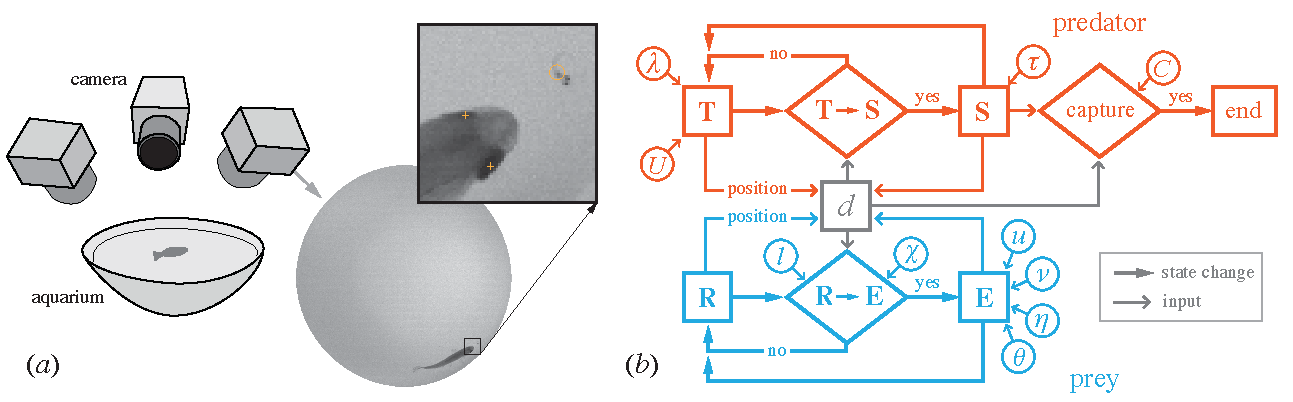
\includegraphics[width=5.5in]{fig_setup}
\caption{
Kinematic measurements and game modeling for studying predator-prey interactions in zebrafish. 
(\textit{a}) Three high-speed video cameras recorded video of one larval prey and one predator fish (adult or juvenile) that were placed in a hemispherical aquarium. 
A representative video frame (cropped to the margin of the aquarium) shows an adult in close proximity to the prey. 
In the inset, orange markers denote the locations of morphological landmarks used to describe the position of the two fish.
This consisted of the position of the two eyes for the predator ("+") and the posterior margin of the swim bladder in the prey (open circle). 
 (\textit{b}) A flow chart illustrates the major components of the game model used to simulate the interactions between predators and prey (see Table \ref{table} for symbol definitions and parameter values). T, S, R, and E represent the Tracking, Striking, Resting, and Escaping states (See section 2d for further explanation).
 }
\label{fig_setup}
\end{figure}

\pagebreak

\begin{figure}[!h]
\centering
	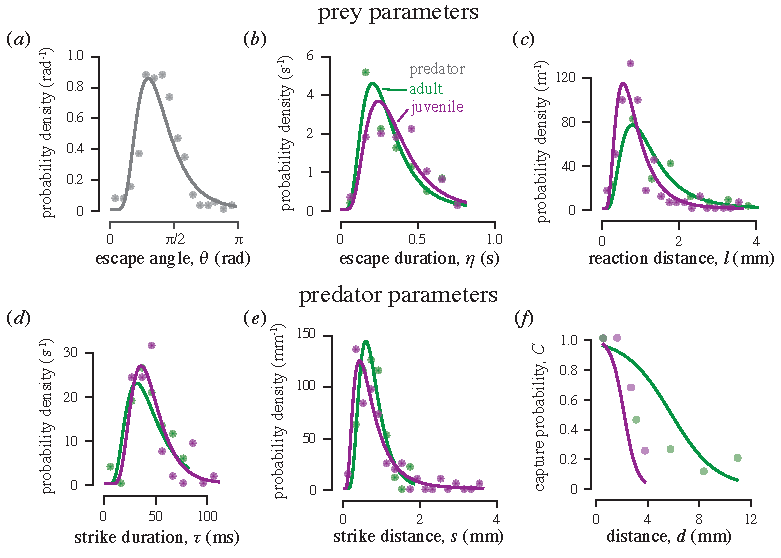
\includegraphics[width=5.5in]{fig_PDFs}
\caption{
Descriptive statistics of swimming kinematics. 
(\textit{a-e}) The probability measurements (circles) and probability density function (Eqn. \ref{eqn_lognorm}) fits for experiments where the predator was a juvenile (purple) or adult (green) predator.
Parameters were measured from the kinematics of prey (\textit{a-c}) and predators (\textit{d-e}).
(\textit{f}) The capture probability was examined as it varies with distance between the predator and prey (Eqn. \ref{eqn_sig}).  
}
\label{fig_PDF}
\end{figure}

\pagebreak

\begin{figure}[!h]
\centering
	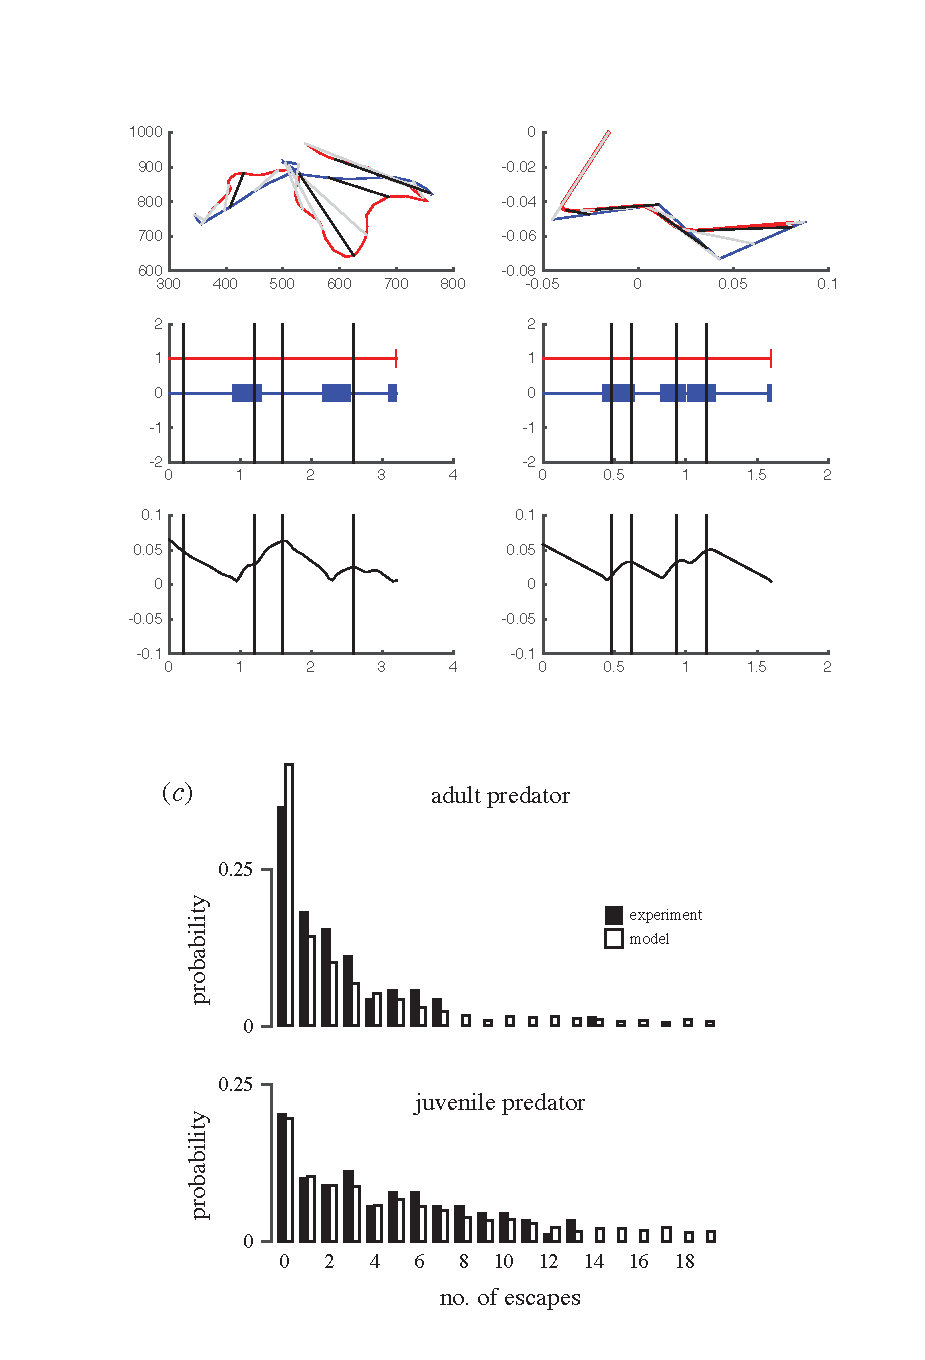
\includegraphics[width=4.5in]{fig_trajectories}
\caption{
Comparison between experimental measurements and game modeling. 
(\textit{a}) Trajectories of predator and prey from a representative experiment (left) and simulation (right). 
The position of predator and prey that correspond to particular time points are shown with connecting arrows.
(\textit{b}) Ethograms for these trajectories illustrate the temporal changes in the predator's swimming and strike (left), which are respectively modeled by the T and S (Fig. \ref{fig_setup}\textit{b}) modes (right). 
The prey's behavior while motionless and during escape (left) were respectively modeled as R and E modes (right).
For both ethograms, the distance between predator and prey are shown.
Particular moments in the trajectories are highlighted with vertical lines that correspond with the same-colored arrows in (\textit{a}).
(\textit{c}) The probability that a prey survives over a particular number of strikes is shown adult  (above) and juvenile (below) predators for experiments (dark gray) and simulations (light gray).   
}
\label{fig_traj}
\end{figure}

\begin{figure}[!h]
\centering
	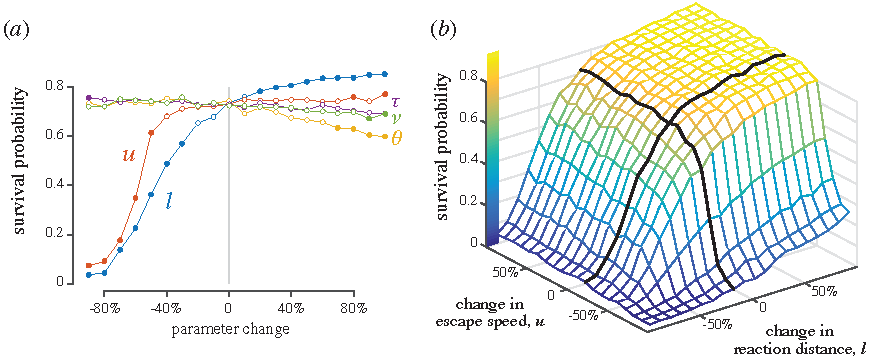
\includegraphics[width=5.5in]{fig_sensitivity}
\caption{Sensitivity analysis of the game model to examine the effects of parameters on escape probability. 
(\textit{a}) We varied the mean of the distribution for each prey parameter by manipulating the log-mean value (see Table \ref{table} for parameter definitions and values), with each point representing the result of 1000 simulations. 
Solid points represent significant differences (KS-test: P < 0.05) from a 0\% change.
(\textit{b}) Variation in escape probability was examined with respect to both escape speed and reaction distance.
The same simulation results are shown with respect to changes in escape speed (\textit{c}) and reaction distance (\textit{d}).
}
\label{fig_sense}
\end{figure}

\pagebreak



\end{document}
